% $Id: appendix.tex 85346 2015-12-15 06:23:34Z pkoppenb $
% ===============================================================================
% Purpose: appendix to the standard template: standard symbol alises from Ulrik
% Author: Tomasz Skwarnicki
% Created on: 2009-09-24
% ===============================================================================

\clearpage

{\noindent\normalfont\bfseries\Large Appendices}

\appendix

\section{Analysis code}\label{sec:app:AnaCode}
 The DecayTreeTuple are made running DaVinci v37r2p4 on the grid. We use Erasmus v10r2. The various steps are:
 \begin{enumerate}
  \item "DTT" with Phys/B2CCtuples/python/BuBdBs$\_$NTUPLE$\_$maker$\_$(2011,2012).py (to change), running DaVinci v37r2p4;
  \item "tupleA" with Phys/B2CCtuples/src/sel1Candidate$\_$Bs2JpsiPhi.C, revison 166293 (to change);\\
  /eos/lhcb/user/v/vbatozsk/B0s2JpsieePhi/\\
  DVNtuples$\_$Bs2JpsieePhiStrip21$\_$TupleBsDetached$\_$RD11$\_$tupleA$\_$new.root\\
 /eos/lhcb/user/v/vbatozsk/B0s2JpsieePhi/\\
 DVNtuples$\_$Bs2JpsieePhiStrip21$\_$TupleBsDetached$\_$RD11$\_$tupleA$\_$new.root
  \item "tupleB" with Phys/B2CCtuples/src/CreateNtupleB.C revision 164683 (to change);\\
 /eos/lhcb/user/v/vbatozsk/B0s2JpsieePhi/\\
 DVNtuples$\_$Bs2JpsieePhiStrip21$\_$TupleBsDetached$\_$RD11$\_$tupleB.root\\
 /eos/lhcb/user/v/vbatozsk/B0s2JpsieePhi/\\
 DVNtuples$\_$Bs2JpsieePhiStrip21$\_$TupleBsDetached$\_$RD11$\_$tupleB.root
 \item  Add physics weights to MC tuples: Phys/B2CCtples/python/mcTuples.py;
 \item  "tupleC" Phys/B2CCtples/python/makeNTupleC.py;
 \item  "final fitting tuple", where the mass sWeights are recomputed dividing the samples in the categories mentioned in the note, with PhysFit/P2VV/examples/createB2CCFitNTuple.py. (to check)
 \end{enumerate}

 The location of the final NTuples are /castor/cern.ch/user/j/jleerdam/JpsiKK$\_$fitNTuples/fitNTuple$\_$peakBkg$\_$2011$\_$2012$\_$Reco14$\_$HLT2B$\_$20140116.root\\
 /castor/cern.ch/user/j/jleerdam/JpsiKK$\_$fitNTuples/fitNTuple$\_$peakBkg$\_$2011$\_$2012$\_$Reco14 $\_$20140116.root. (to change)
\clearpage

\section{Data/MC comparison}\label{sec:app:DataMC}
 
 \begin{figure}[htb]
  \begin{center}
    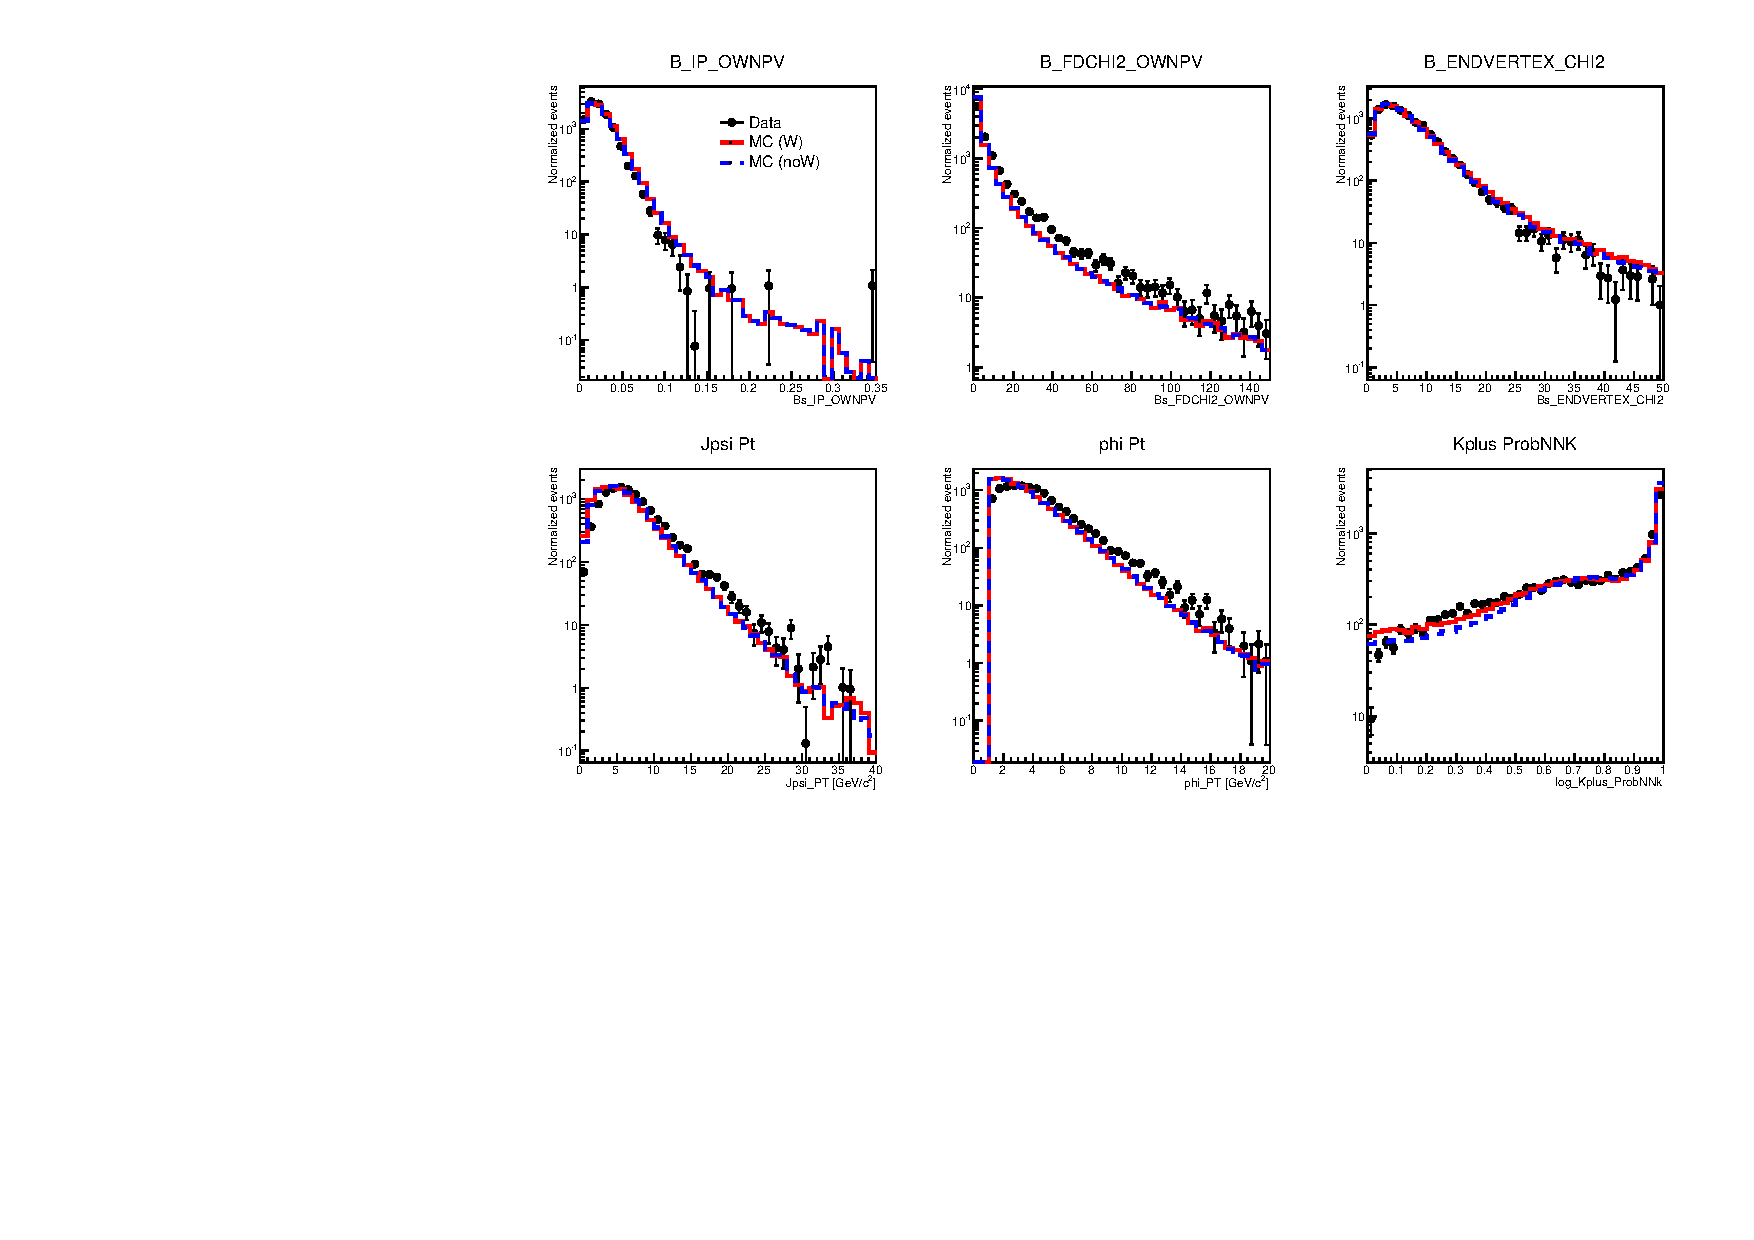
\includegraphics[width=1\linewidth]{Data_MC/Data_MC_W_noW1.pdf} \\
  \end{center}
  \caption{
   Data({\it $_{s}$Plot})/MC comparison for $\Bs\to\jpsi(e^{+}e^{-})\phi$. All distributions are in logarithmic scale.
}
  \label{fig:app:DataMC1}
\end{figure}
 \begin{figure}[tb]
  \begin{center}
    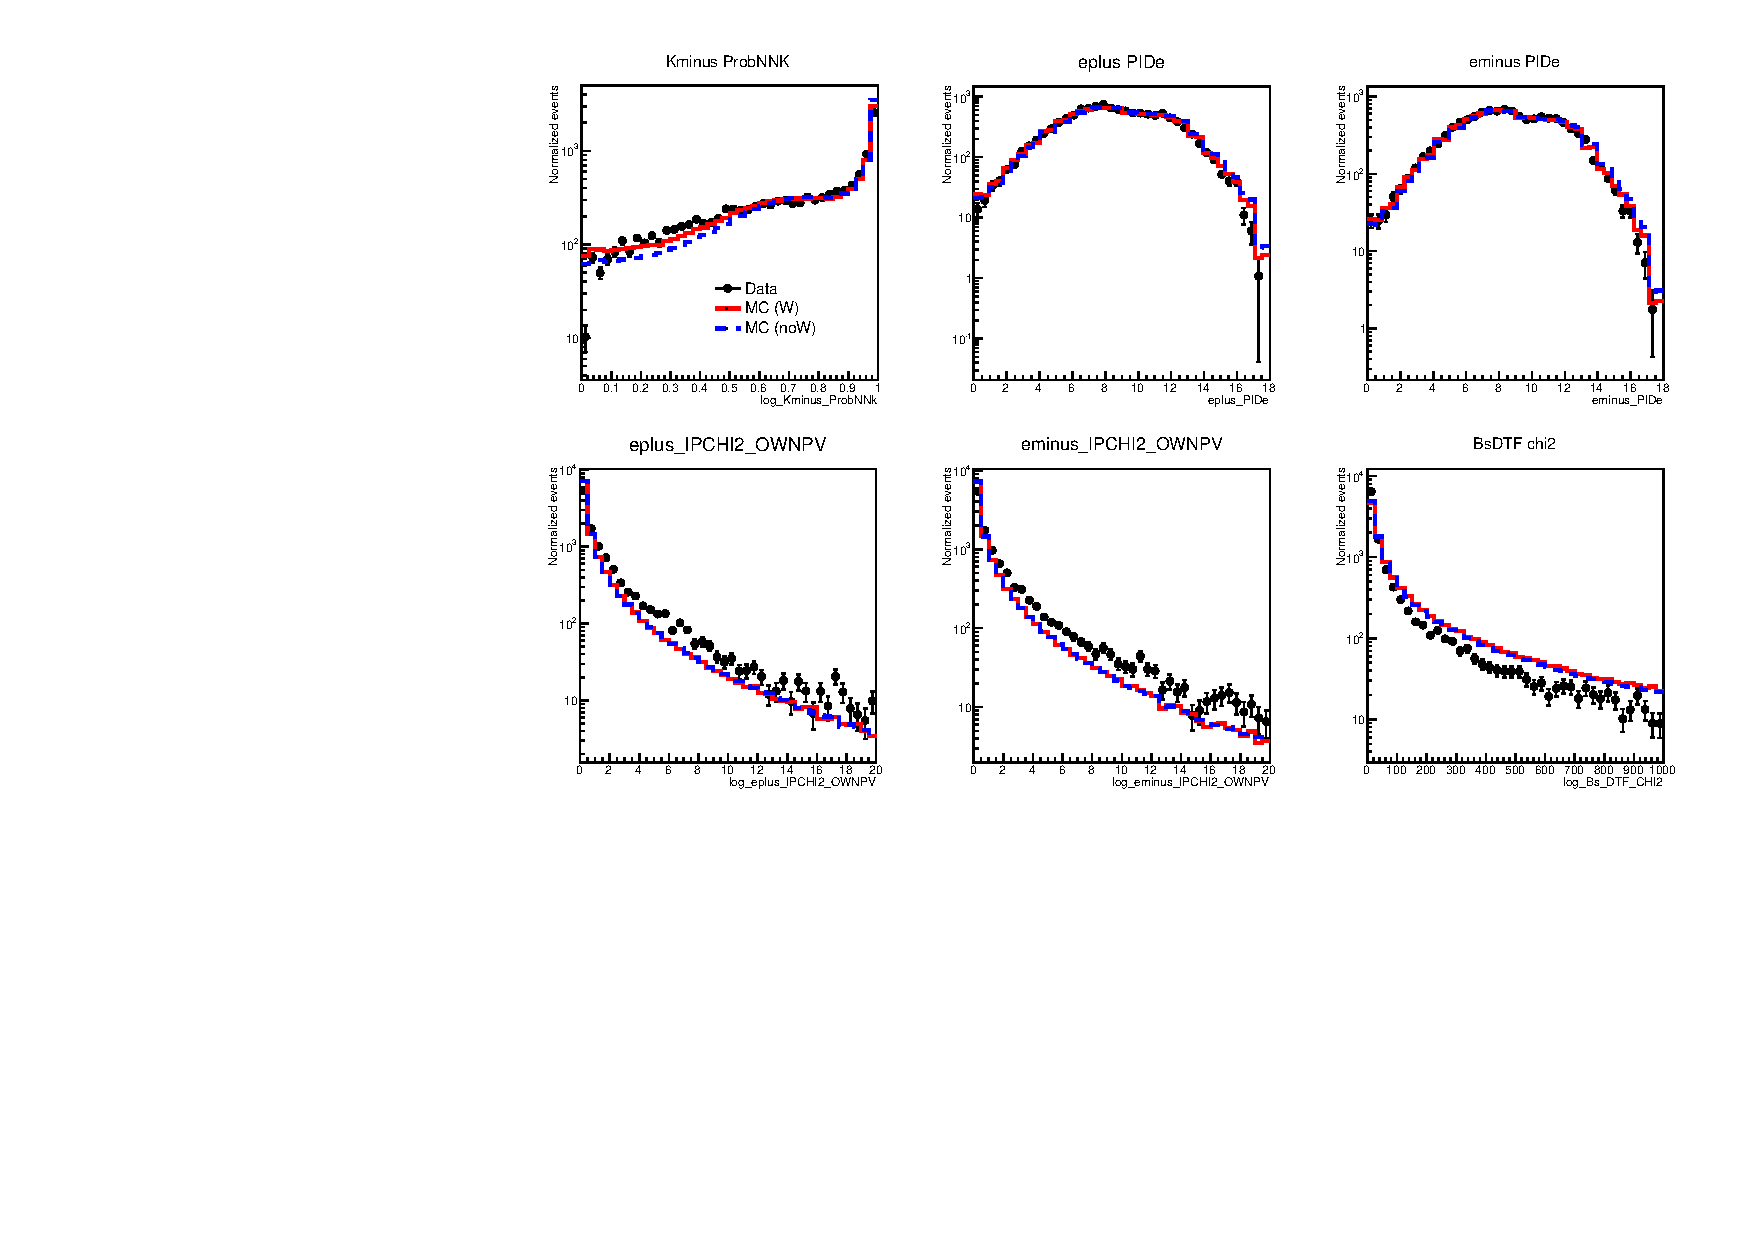
\includegraphics[width=1\linewidth]{Data_MC/Data_MC_W_noW2.pdf} \\
  \end{center}
  \caption{
   Data({\it $_{s}$Plot})/MC comparison for $\Bs\to\jpsi(e^{+}e^{-})\phi$. All distributions are in logarithmic scale.
}
  \label{fig:app:DataMC2}
\end{figure}
 \begin{figure}[tb]
  \begin{center}
    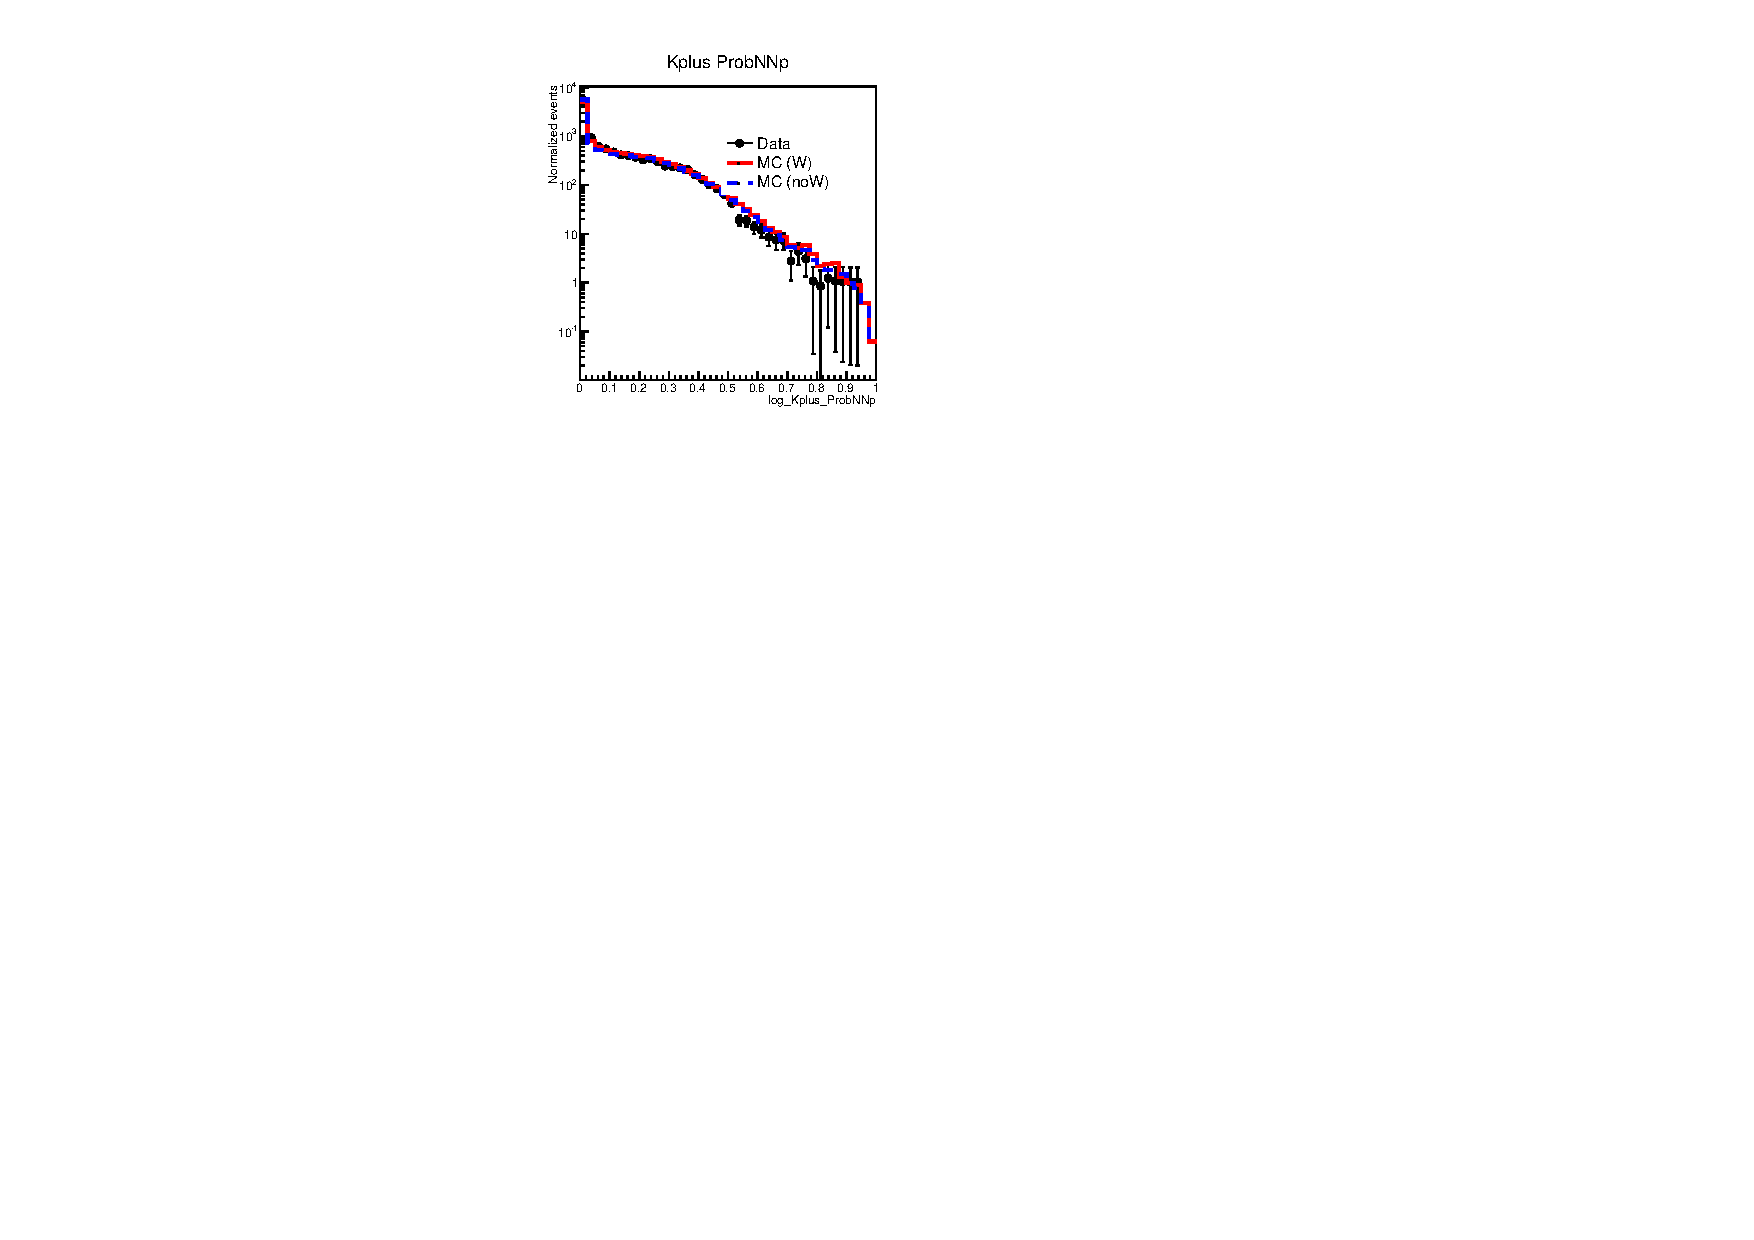
\includegraphics[width=1\linewidth]{Data_MC/Data_MC_W_noW3.pdf} \\
  \end{center}
  \caption{
   Data({\it $_{s}$Plot})/MC comparison for $\Bs\to\jpsi(e^{+}e^{-})\phi$. All distributions are in logarithmic scale.
}
  \label{fig:app:DataMC3}
\end{figure}
 \begin{figure}[tb]
  \begin{center}
    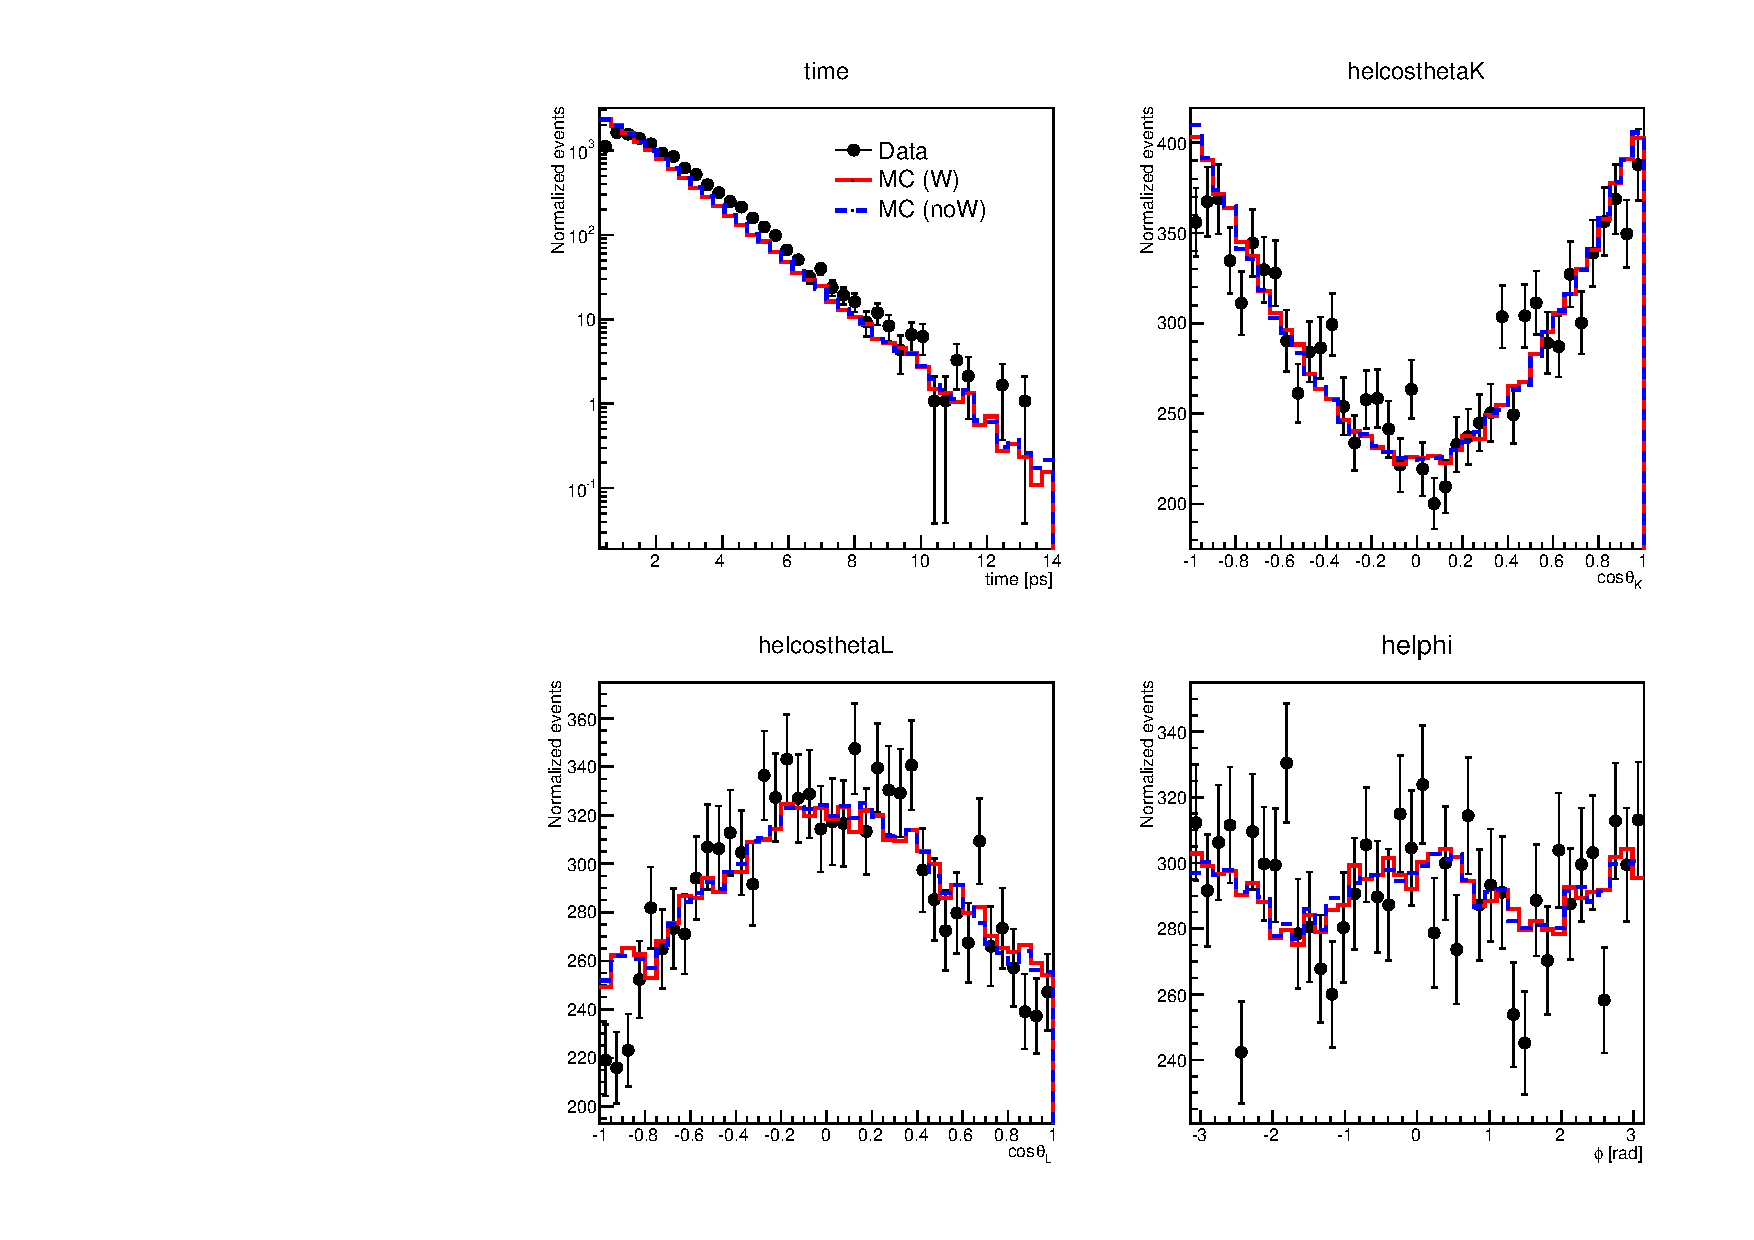
\includegraphics[width=0.9\linewidth]{Data_MC/Data_MC_W_noW4.pdf} \\
  \end{center}
  \caption{
   Data({\it $_{s}$Plot})/MC comparison for $\Bs\to\jpsi(e^{+}e^{-})\phi$. The decay time distribution are in logarithmic scale.
}
  \label{fig:app:DataMC4}
\end{figure}

\clearpage

\section{BDT training}\label{sec:app:BDT}
\subsection{Boosted Decision Tree}

 This section includes the details of the BDT used for the final step of selection (Sec.~\ref{subsec:BDT}). The list of variables used is shown in Table~\ref{tab:RankingBDT}. Plots showing the distributions of the input variables from TMVA are shown in Figure~\ref{fig:BDTvariables}.
 \begin{figure}[htb]
  \begin{center}
    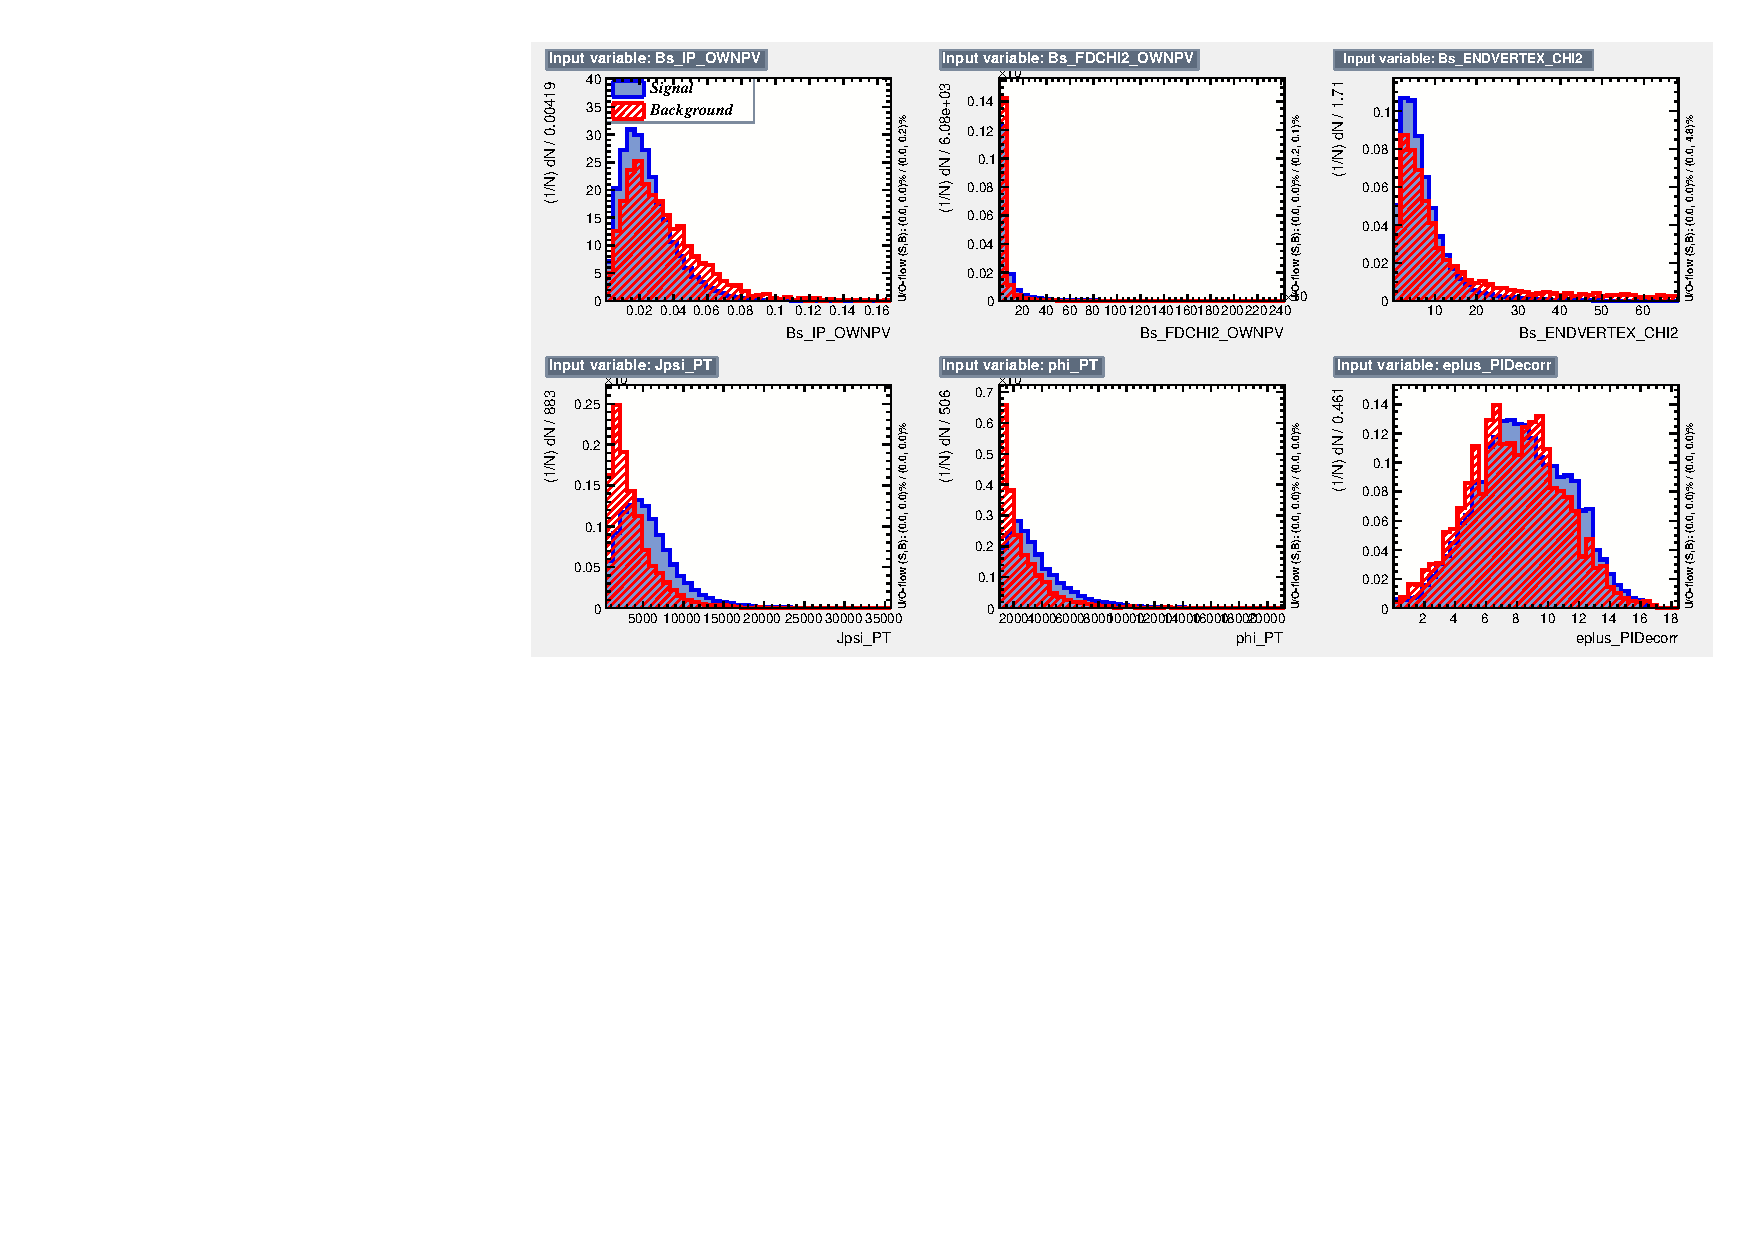
\includegraphics[width=0.9\linewidth]{BDT/input_variables1_bkgcat0_wSPDHits_trigger_RD12.pdf} \\
    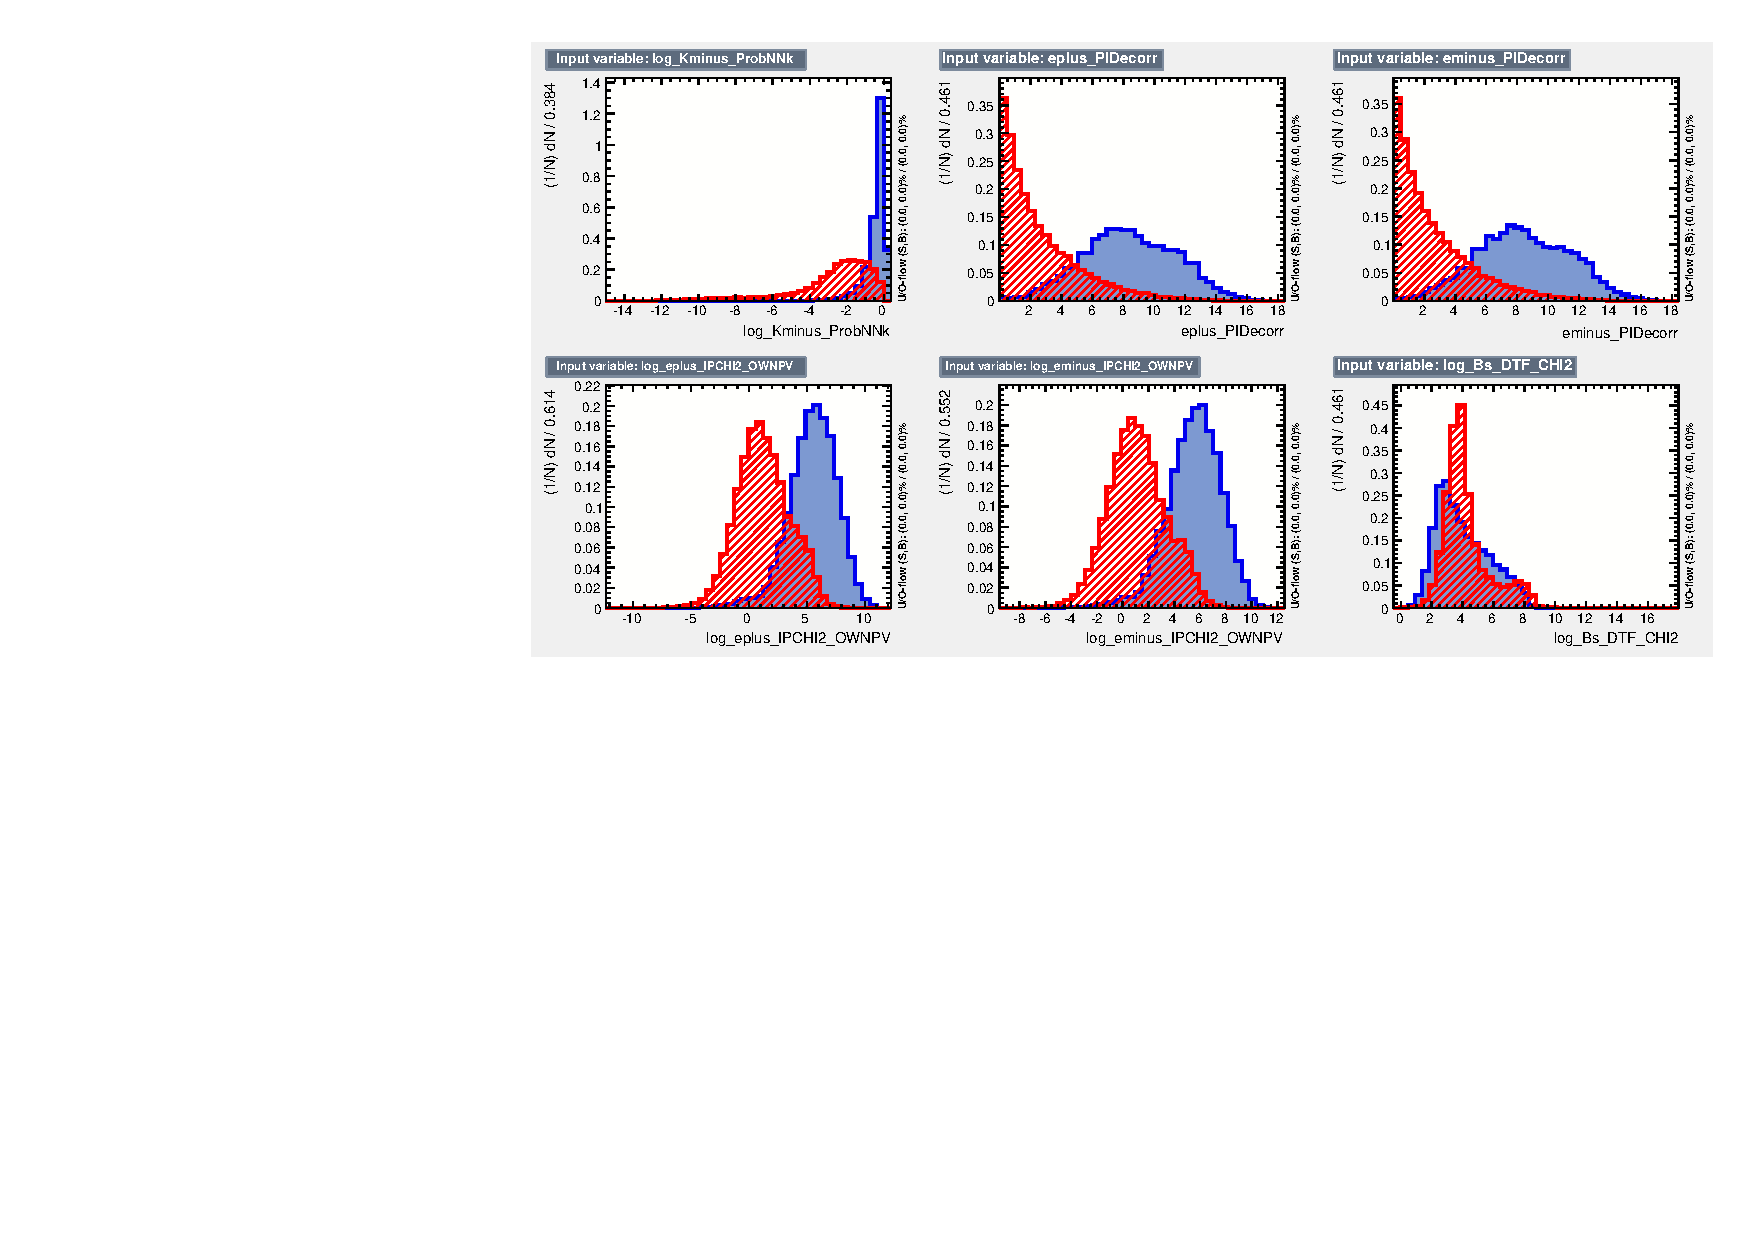
\includegraphics[width=0.9\linewidth]{BDT/input_variables2_bkgcat0_wSPDHits_trigger_RD12.pdf} 
  \end{center}
  \caption{
   Input variable distributions for signal (blue) and background (red) for the 2012 BDT training.
}
  \label{fig:BDTvariables}
\end{figure}

\subsection{Peaking background}

 This section includes the details of second BDT used to reduce background under $\Bs$ mass peak (Sec.~\ref{subsec:PeakBkg}). The list of variables used is shown in Table~\ref{tab:RankingBDT2}. Plots showing the distributions of the input variables from TMVA are shown in Figure~\ref{fig:BDTvariables2}.
 \begin{figure}[htb]
  \begin{center}
    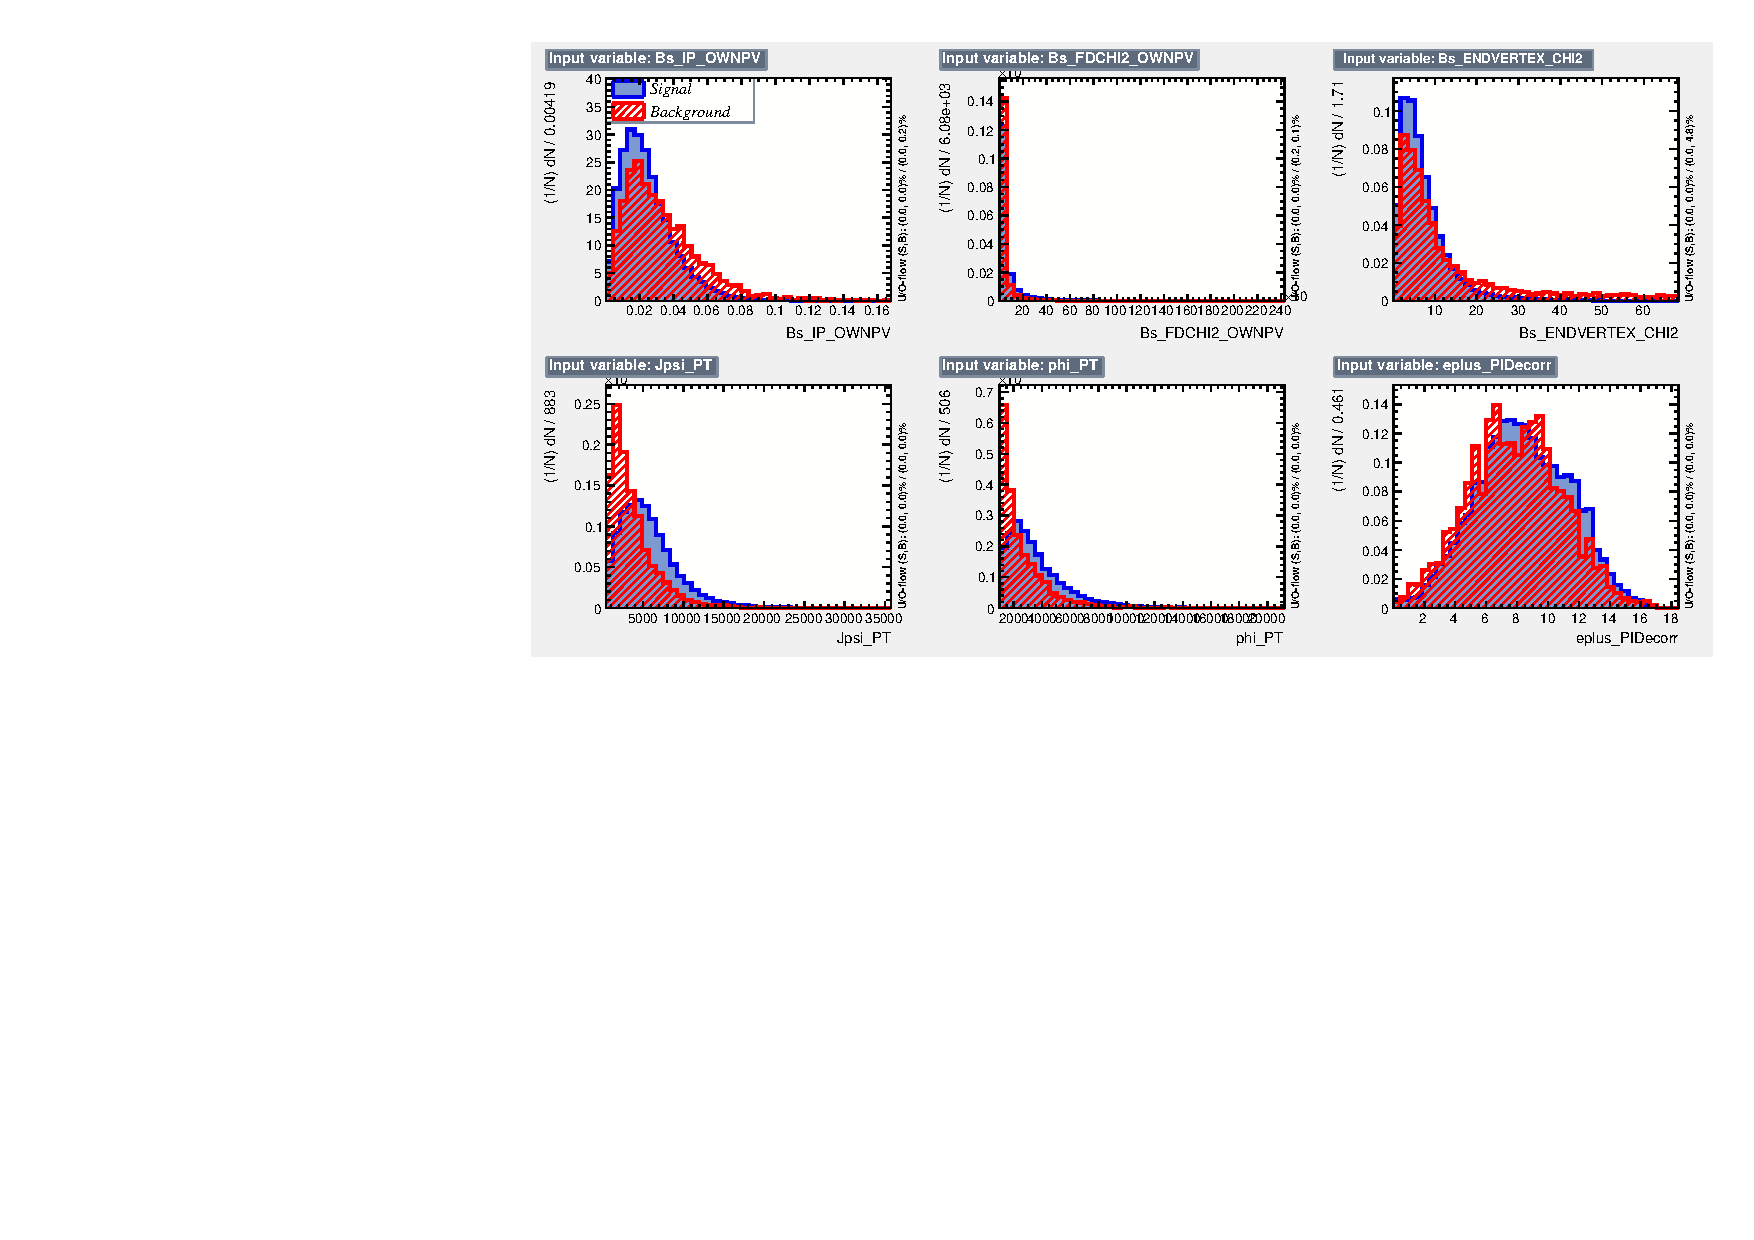
\includegraphics[width=0.9\linewidth]{BDT/input_variables1_Lb_bkgcat0_wSPDHits_trigger_RD12.pdf} \\
    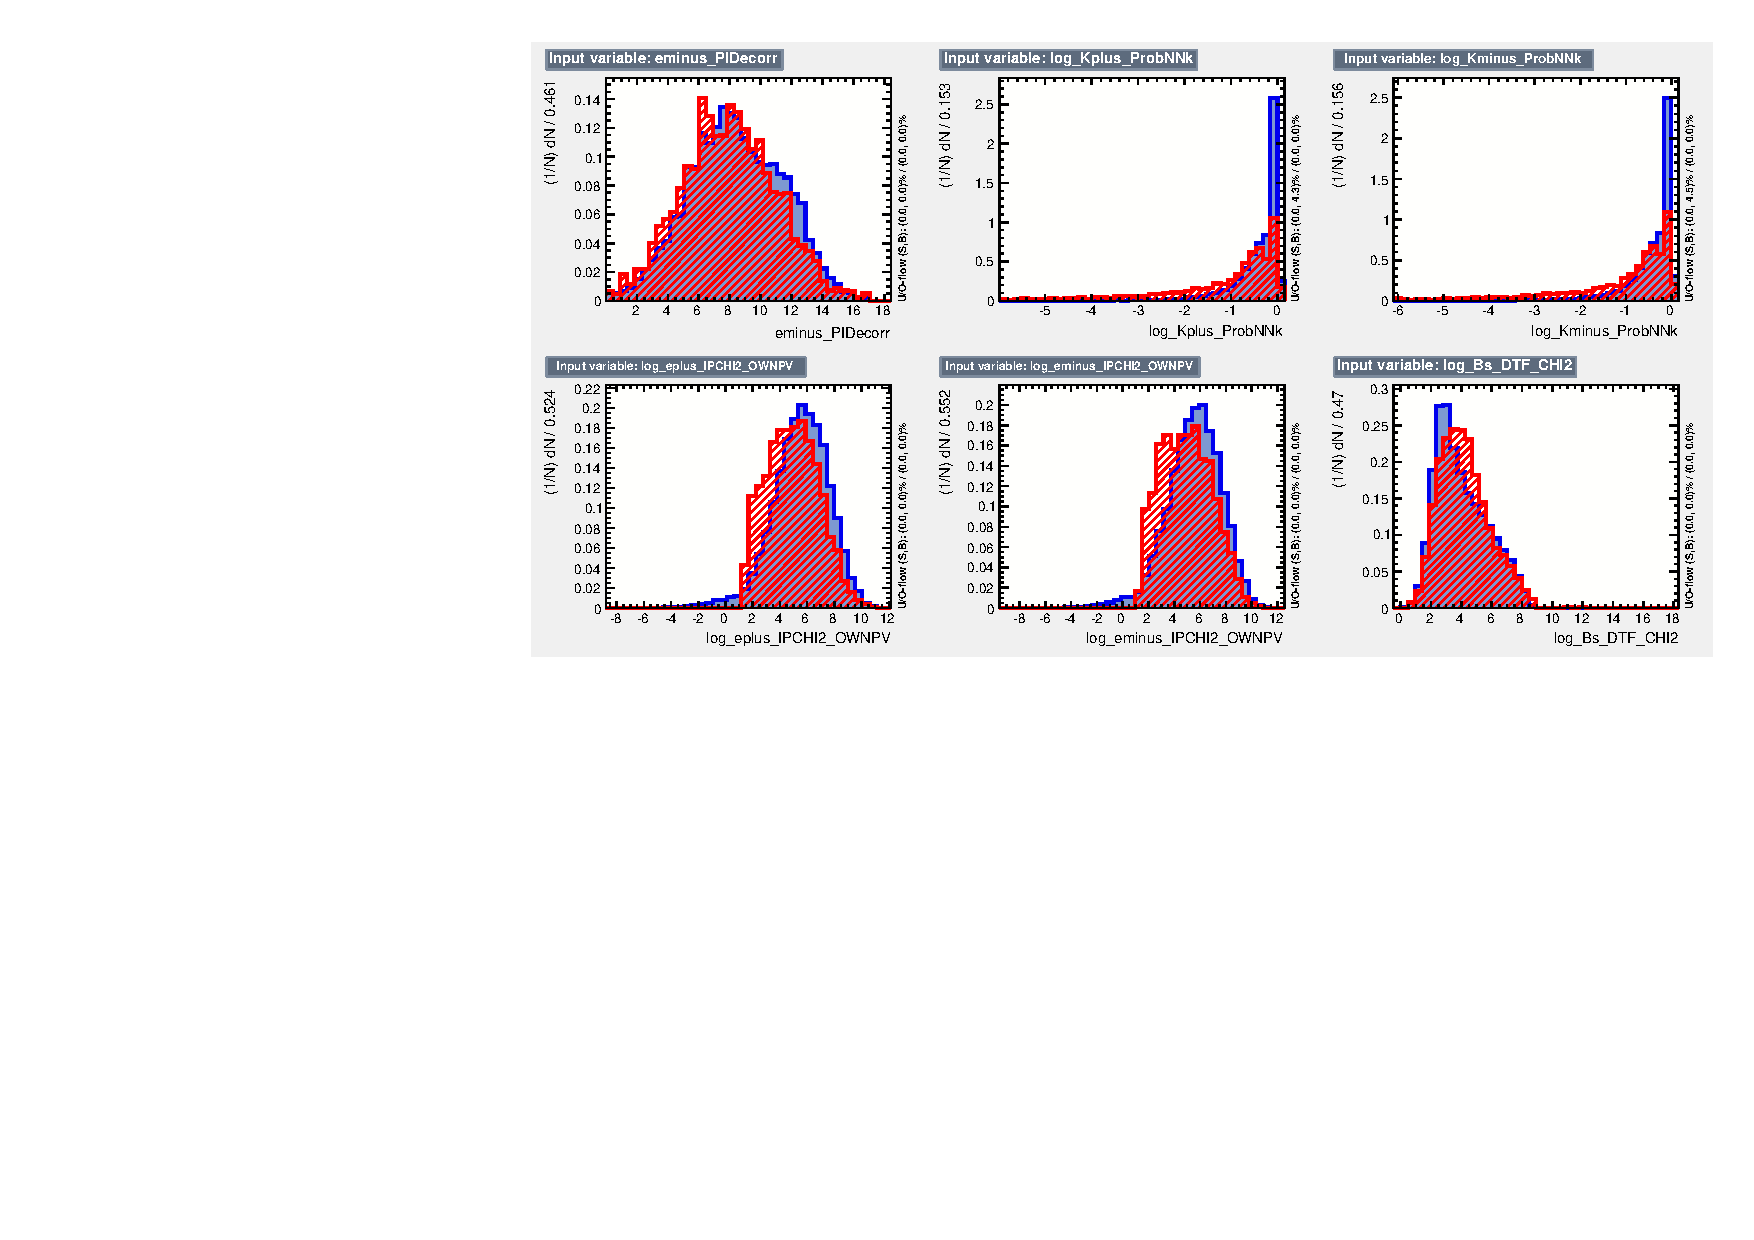
\includegraphics[width=0.9\linewidth]{BDT/input_variables2_Lb_bkgcat0_wSPDHits_trigger_RD12.pdf} \\
  \end{center}
  \caption{
   Input variable distributions for signal (blue) and background (red) for the 2012 BDT training.
}
  \label{fig:BDTvariables2}
\end{figure}
 \begin{figure}[htb]
  \begin{center}
    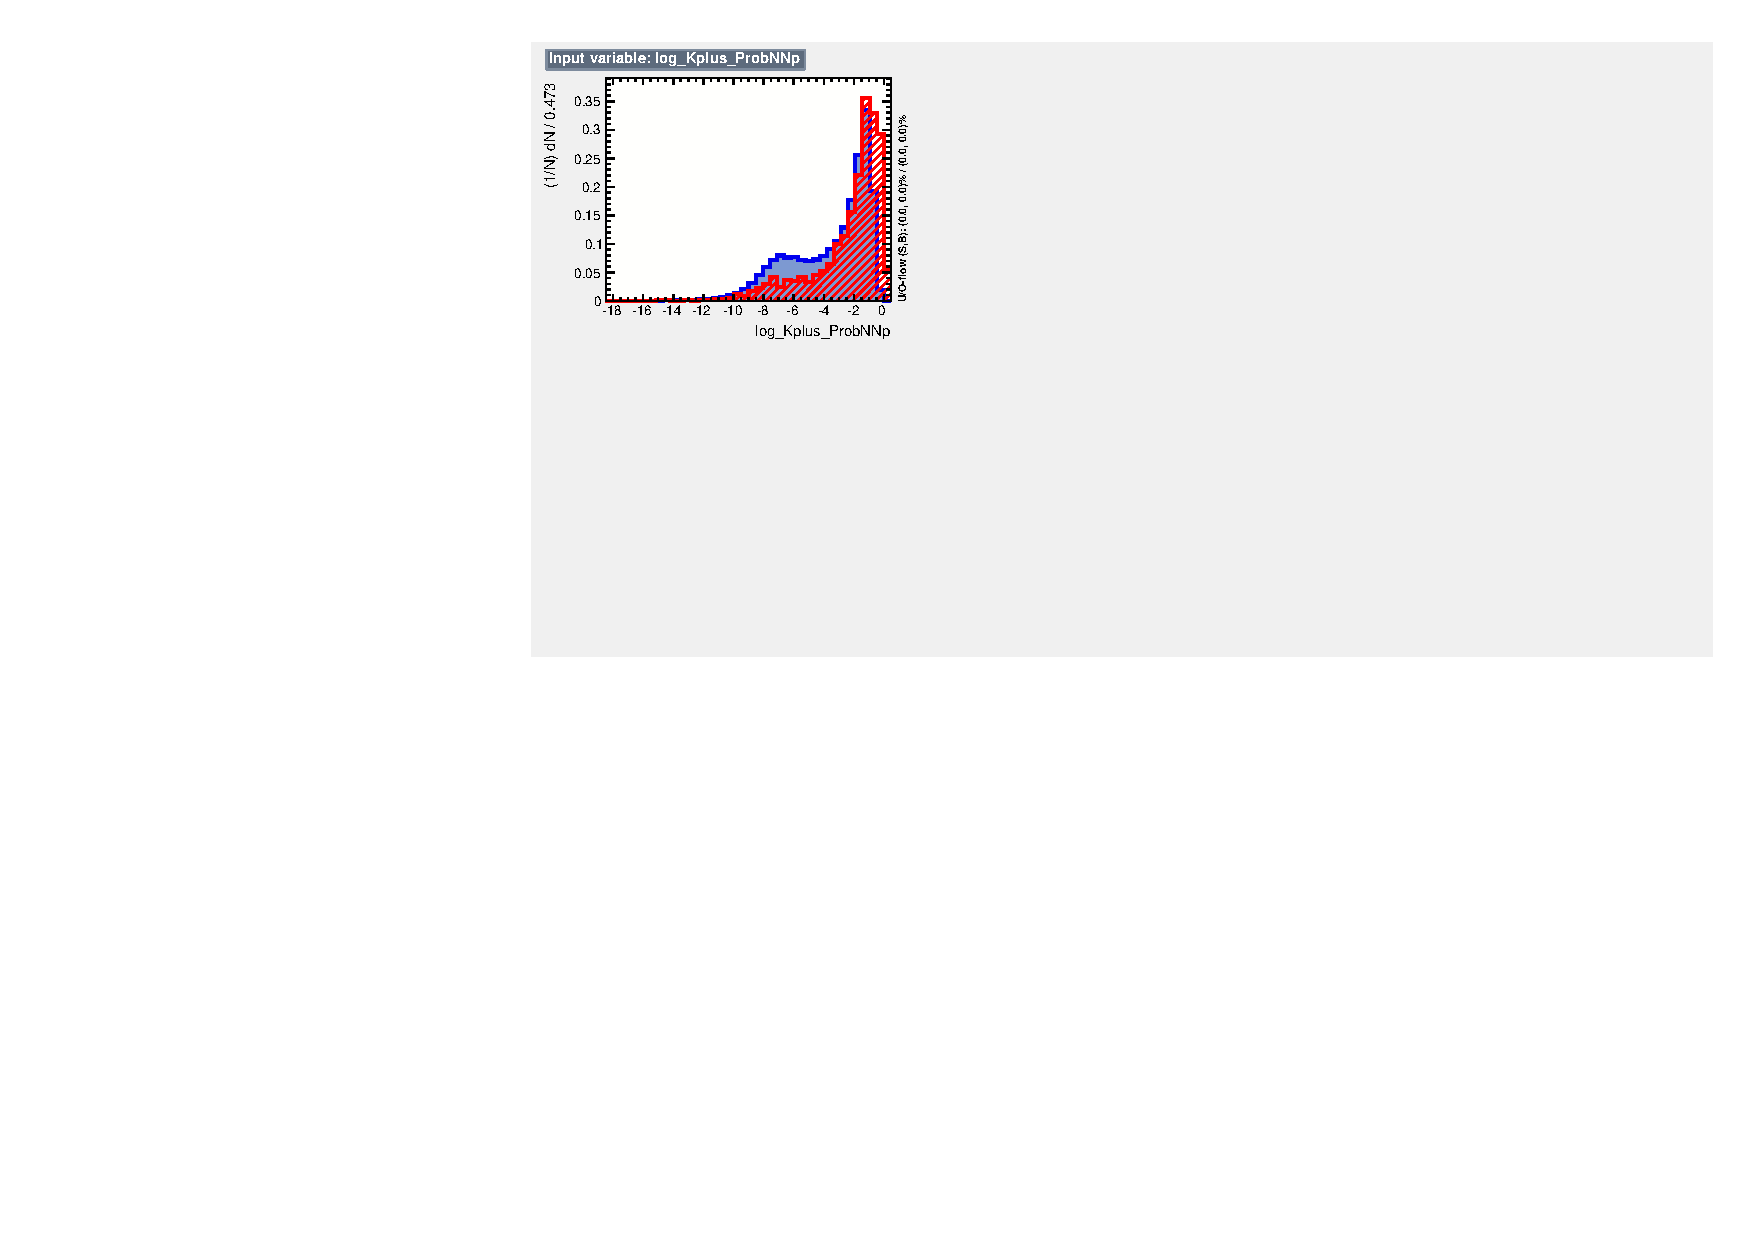
\includegraphics[width=0.9\linewidth]{BDT/input_variables3_Lb_bkgcat0_wSPDHits_trigger_RD12.pdf}
  \end{center}
  \caption{
   Input variable distributions for signal (blue) and background (red) for the 2012 BDT training.
}
  \label{fig:BDTvariables2_1}
\end{figure}

\clearpage

\section{Comparison of $\Bs\to\jpsi(\mumu)\Kp\Km$ and $\Bs\to\jpsi(\epem)\phi$ distributions}\label{sec:app:Comparison}

 \begin{figure}[htb]
  \begin{center}
    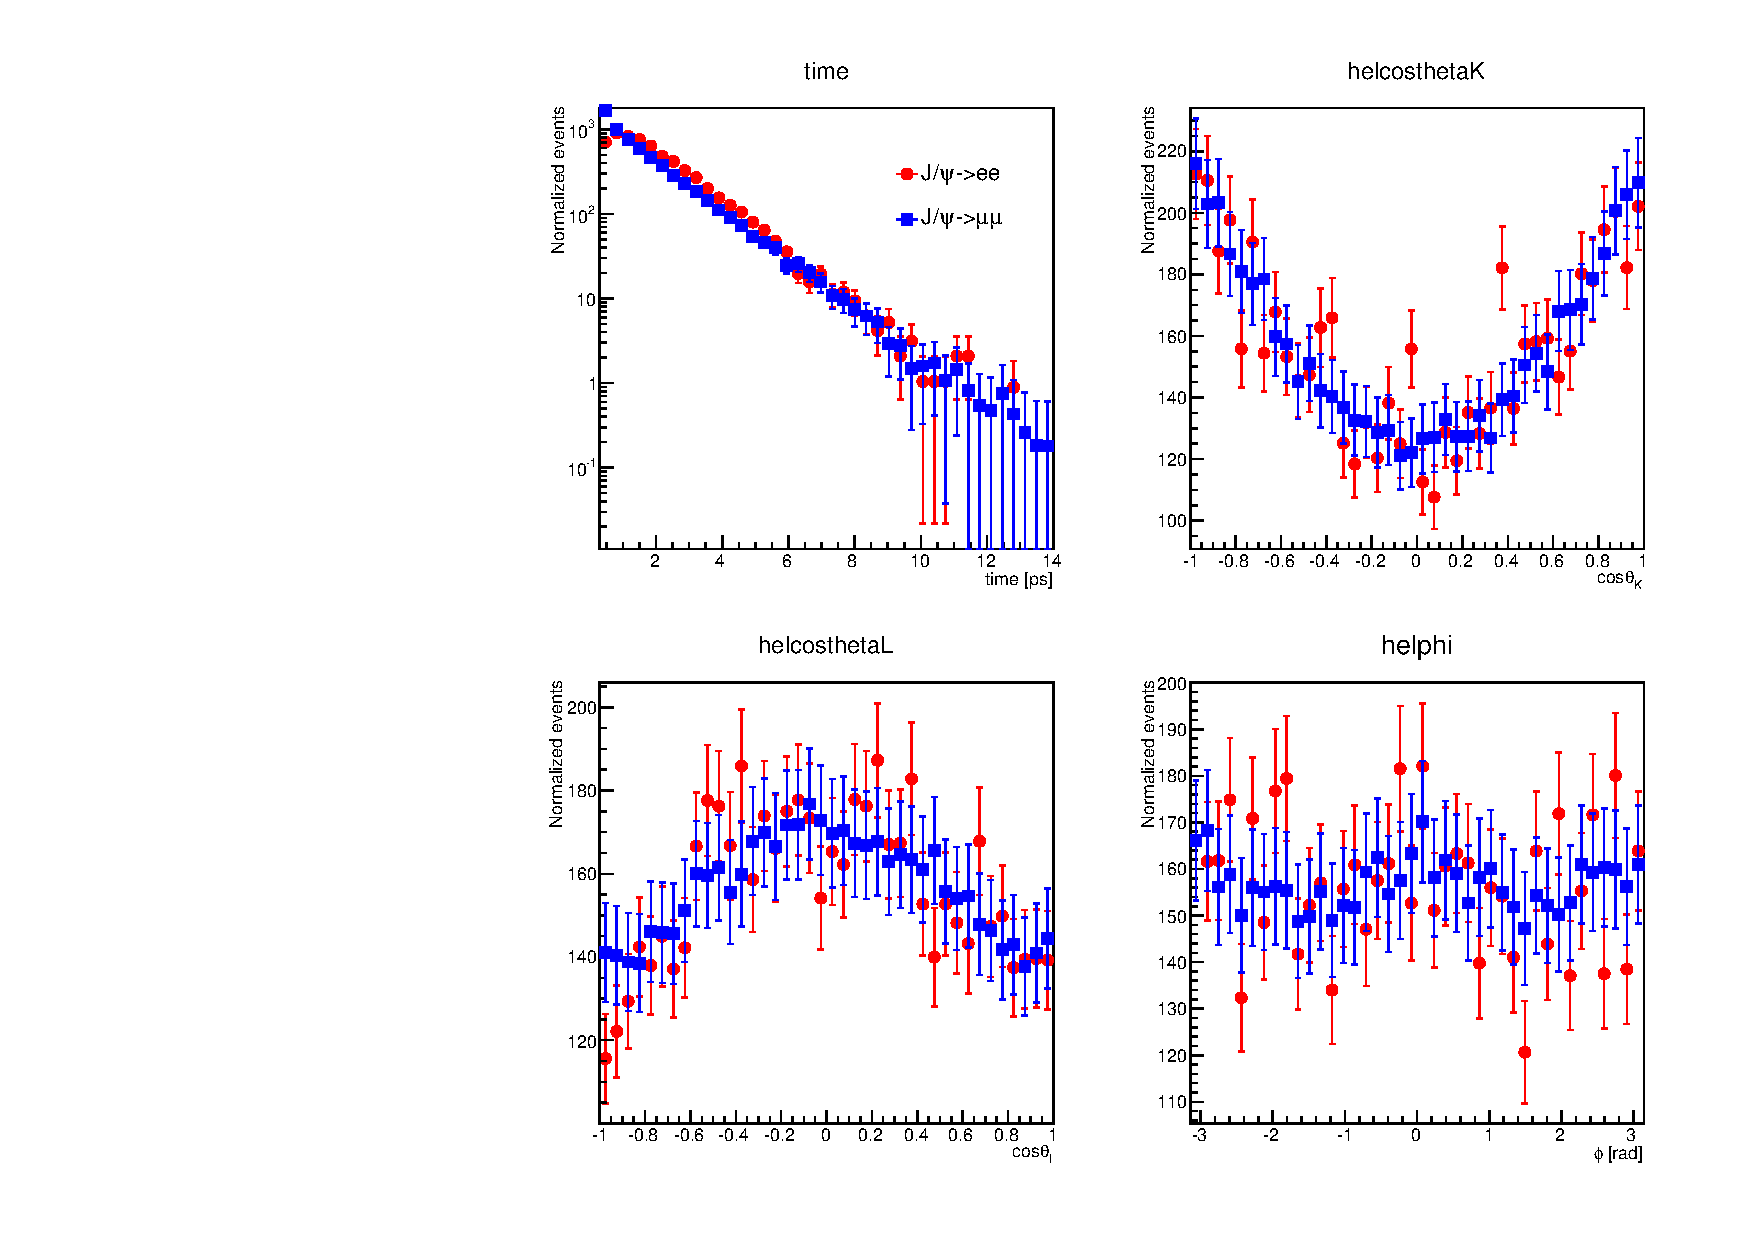
\includegraphics[width=0.9\linewidth]{Data_ee_MuMu/time_angles.pdf} \\
  \end{center}
  \caption{
   Plot of the decay time and helicity angles for sWeighted $\Bs\to\jpsi(\epem)\phi$ data (red) and sWeighted $\Bs\to\jpsi(\mumu)\Kp\Km$ data (blue).
}
  \label{fig:BDTvariables}
\end{figure}
\clearpage